\section{Introduction}
Autonomous mobile robots (AMRs), from robotaxis \cite{waymo} to platform, towing, and goods-to-person AMRs \cite{abb_flexley_mover}, routinely operate in narrow hallways, single-lane passages, and warehouse aisles where two robots cannot pass side by side \cite{fragapane2021planning,xiao2022barn}. When two robots meet head-on in such an aisle (Fig.~\ref{fig:narrow_corridor_examples}), slowing down or swerving is not enough: one robot must yield, reversing into a pull-in bay or out of the corridor, usually at reduced speed and with degraded rear sensing.

Existing approaches are either decentralized or centralized. Decentralized controllers based on velocity obstacles \cite{vandenberg2011orca} or control barrier functions (CBFs) \cite{wang2017safety,grover2023before} need no messages but fall into symmetric deadlocks in narrow head-on configurations \cite{grover2023before,dergachev2021distributed,zheng2023deadlock,chandra2025deadlock}; such standoffs have been reported anecdotally in public robotaxi deployments \cite{stuff_robotaxi_standoff,nyt_waymo_honking}. Centralized methods, including multi-agent path finding (MAPF) \cite{sharon2015cbs,stern2019mapf,okumura2022pibt}, zone-control locks \cite{fanti2002event}, and fleet managers such as Open-RMF \cite{openrmf} and VDA~5050 \cite{vda5050}, prevent conflicts globally but assume a common map, reliable connectivity, and a single coordinating authority, which ad hoc deployments, radio-shadowed aisles, and multi-vendor facilities violate \cite{gautier2022negotiated,gielis2022critical}.

\begin{figure}[!t]
  \centering
  \subfloat[Single-track road \cite{robson2013singletrack}.]{%
    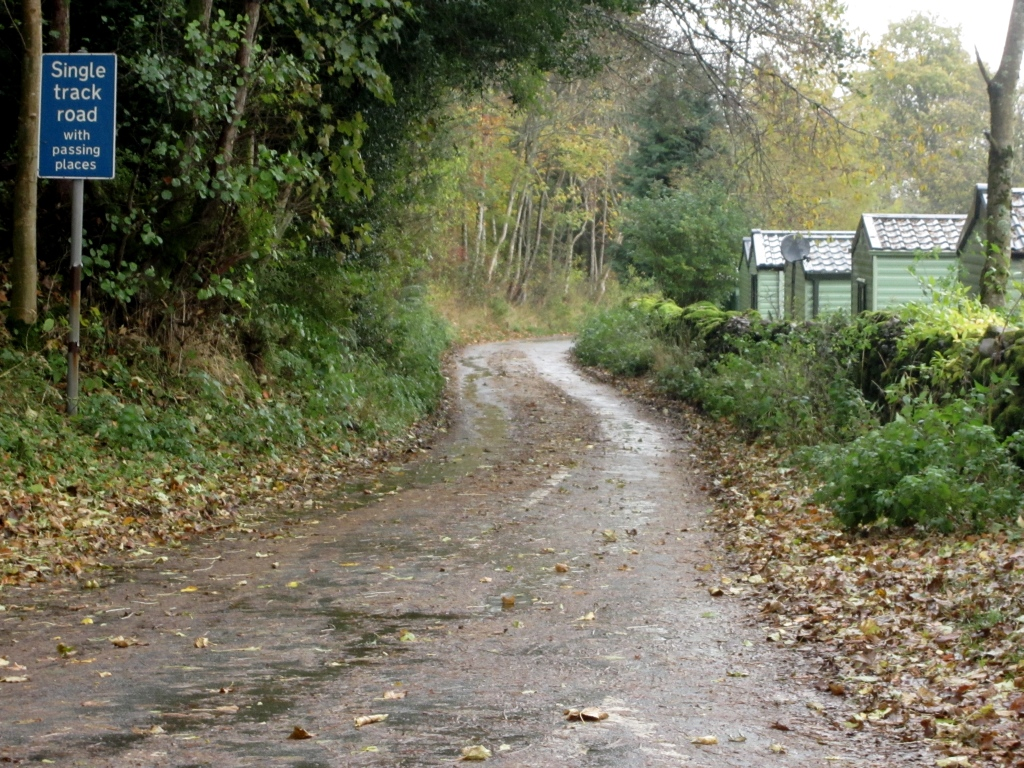
\includegraphics[width=0.485\columnwidth,trim=0 65 0 12,clip]{Images/road_example.jpg}%
  }\hfill
  \subfloat[Warehouse aisle with AMR \cite{dematic_radial_amr}.]{%
    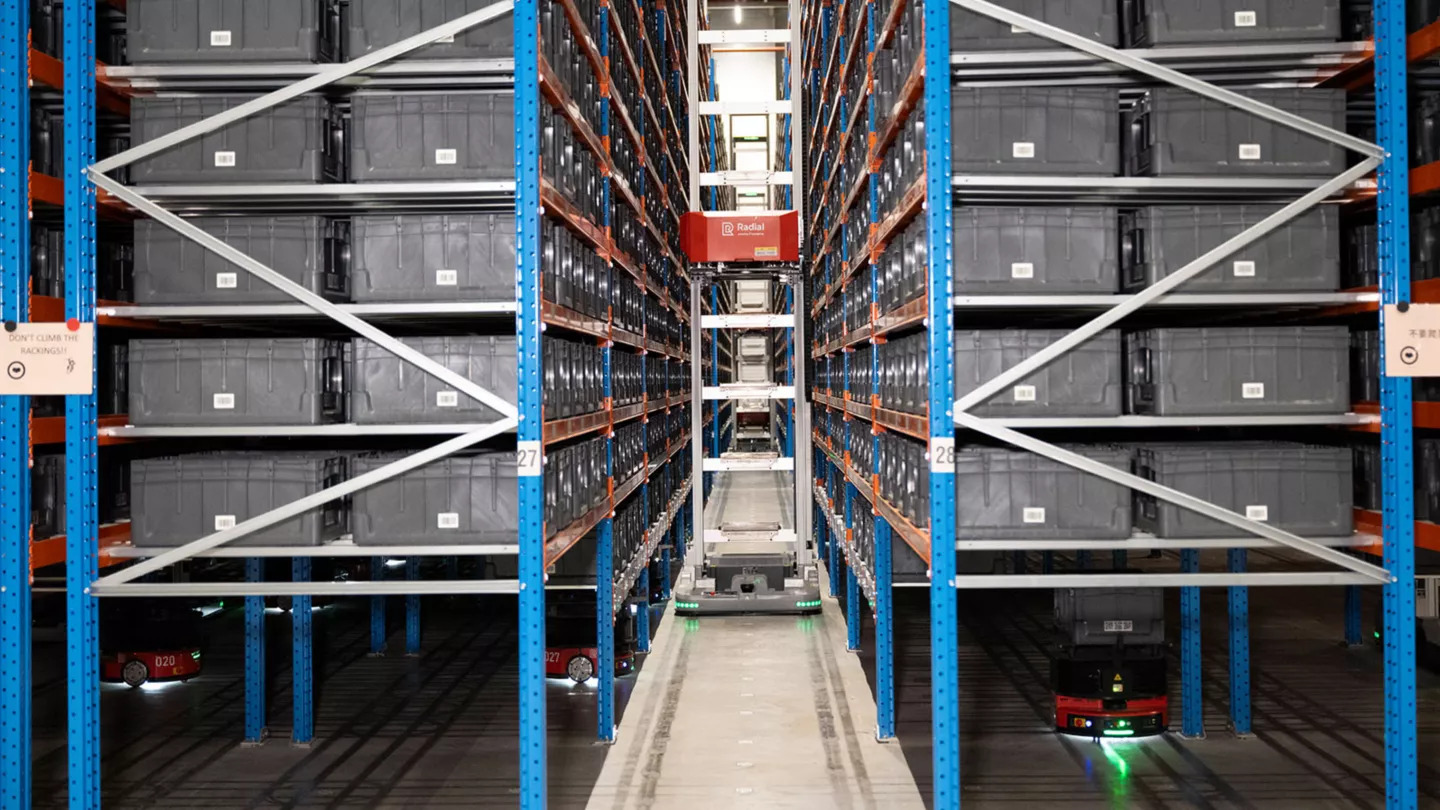
\includegraphics[width=0.485\columnwidth]{Images/warehouse_example.jpg}%
  }
  \caption{Single-lane environments where two vehicles cannot pass side by side: (a) public road with passing places (photo: G.~Robson, CC BY-SA 2.0); (b) high-density warehouse aisle (image courtesy of Dematic, used with permission).}
  \label{fig:narrow_corridor_examples}
\end{figure}

An alternative is decentralized peer-to-peer negotiation: encountering robots exchange compact messages over a local broadcast channel and agree on who yields and into which refuge, keeping infrastructure-free operation while breaking symmetric deadlocks (in contrast to infrastructure-based prescriptive collaboration \cite{george2025infrastructure}). Candidate mechanisms include social laws and rulebooks \cite{kato1992coordinating,shoham1995social,censi2019rulebooks}, auctions \cite{gerkey2002sold,gautier2022negotiated}, incentive-compatible mechanisms for MAPF and robot prioritization \cite{amir2015mapfauction,das2021omcorp,friedrich2024scalable}, karma economies \cite{censi2019karma,elokda2024karma}, learned give-way policies \cite{bettini2022vmas,bettini2023heterogeneous,park2023hallucination}, and language-model negotiators \cite{marlin2024,gamechat2025,garg2024llm}. Three gaps remain \cite{chandra2026social,francis2025principles}.
\begin{enumerate}
\item \emph{No shared refuge-and-reversing benchmark across policy families.} Corridor give-way studies, including MARLIN's single- and two-slot corridors \cite{marlin2024}, VMAS \texttt{give\_way} \cite{vmasgiveway}, and narrow-hallway navigation \cite{park2023hallucination,alghamdi2025opinion}, each evaluate one or two policy families. To our knowledge, none compares rule-based, lock-based, market-based, mechanism-design, and learned policies on one geometry with nonholonomic turn-and-park maneuvers, asymmetric reverse speeds, and multiple bays (Table~\ref{tab:relwork}).
\item \emph{Siloed assumptions on information, incentives, and channels.} Rulebooks assume cooperative agents, auctions assume truthful costs, mechanism-design studies assume lossless single-shot games, and loss-tolerant protocols are rarely benchmarked against a per-encounter reference.
\item \emph{Unverified 2D-to-3D transfer.} Fast 2D simulators make large sweeps cheap but are rarely checked against a physics simulator running the same software, where perception must infer the peer from Lidar and messages arrive asynchronously. This paper checks transfer to Gazebo with ground-truth localization; hardware remains future work.
\end{enumerate}
We address these gaps with one benchmark organized in two layers: a decision layer that decides who yields and where (RQ1--RQ2), and an execution layer that carries the decision out under wireless loss, map errors, and 3D physics (RQ3--RQ4).
\begin{enumerate}
\item[RQ1] How much delay do rulebooks, learned lookups, and kinematic cost bidding save over reactive backoff and corridor locking, and at what cost-estimation error do rules catch up with bidding?
\item[RQ2] How easily can self-interested robots game unpriced or direct-transfer auctions, what do Clarke-pivot payments cost in budget and collusion, and how cheaply can delay credits balance repeated encounters?
\item[RQ3] How does broadcast negotiation behave under extreme and correlated packet loss, which safeguards prevent collisions, and how can robots recover from incomplete or obstructed bay maps?
\item[RQ4] Which primitives prevent deadlocks in 2-vs.-1 convoys and three-robot T-junctions, and where do 2D predictions diverge from ROS~2/Gazebo execution?
\end{enumerate}

This paper makes four contributions.
\begin{enumerate}
\item Benchmark and dataset. An open ROS~2 benchmark runs one 20\,Hz agent controller in a fast 2D simulator and in Gazebo Harmonic across six corridor topologies (Fig.~\ref{fig:scen}), with 26 studies ($123{,}024$ 2D episodes) and 496 seed-paired Gazebo runs, released with per-episode data, commit hashes, and reproduction commands.
\item Decision-layer characterization (RQ1--RQ2). Nine policies are compared against the better forced-yielder outcome across geometries and heterogeneous fleets, random and systematic cost error, strategic misreporting with shared and private types, and repeated encounters.
\item Protocol ablation and map primitives (RQ3). Three safeguards are ablated under $90$--$99\%$ independent, bursty, and blackout loss. Collision-freedom comes from the local Lidar and timer layer, to which robots often fall back, and piggybacking known bay lists on \texttt{BID} messages removes incomplete-map penalties without extra packets.
\item Multi-robot extensions and Gazebo audit (RQ4). Follower backoff (\texttt{make\_room}), convoy bidding (\gb), and junction staging (\texttt{goal\_wait}) extend pairwise negotiation to convoys and T-junctions. In Gazebo, $97.0\%$ of 406 negotiating runs reproduce the 2D yield choice and straight-corridor excess delays match within $1.0$\,s, whereas T-junction delays do not transfer.
\end{enumerate}

Section~\ref{sec:rel} reviews related work, Section~\ref{sec:problem} formulates the encounter, Section~\ref{sec:exp} describes the protocol, policies, and experimental design, Section~\ref{sec:results} presents results for RQ1--RQ4, Section~\ref{sec:disc} distills guidelines and limitations, and Section~\ref{sec:conc} concludes. Extended results, notation, parameters, and reproduction details are in the supplementary material.